%!TEX root = ../report.tex
\section{Architectural vision}
\begin{figure}[hb!]
%\centering
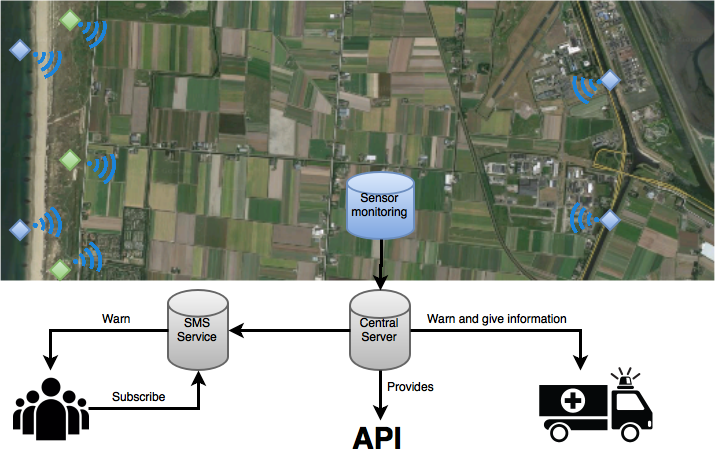
\includegraphics[keepaspectratio=true,width=0.9\textwidth]{images/archVision.png}
\caption{Schematic overview of the flood monitoring system}
\label{fig:architectural-vision}
\end{figure}

The smart flood monitoring system consists of multiple parts. These are represented in figure \ref{fig:architectural-vision}. First of all there is the monitoring part. This part monitors the current state of the environment. To achieve this, we need a lot of data. This data is obtained by sensors,weather data and UAV's. We use sensors to get the current water level of waterways, these water sensors are shown in the figure as blue squares. We also measure the density and structure of dikes, this is done by pressure meters, temperature meters and tilt meters. These are represented as green squares. To see how far a flood has spread we use UAV's. The data that is obtained through all sensors will be send to the central server. Here the information will be processed. The system then determines if there is an imminent flood.

In case of an imminent flood a warning will be issued to the government and the citizens who live in the threatened area. We do this by issuing a warning to the government. In their turn the government uses their infrastructure to warn the citizens. In the Netherlands this infrastructure consists of a siren system and an SMS-system. Besides this people can also apply for our SMS service. People who are subscribed to this service will receive a text message with more information about the imminent flood. 

If people want to have more information on an imminent flood, they can always access the API. This API gives relevant raw data about imminent floods. To make a usable interface for the citizens, we want to cooperate with third party developers. These developers could create an application that can guide citizens to a save area.
%http://www.waterforum.net/Artikel/PrintArtikel.aspx?ID=9132
